
% Change dir here
\def\covmac{/Users/matiascovarrubias/Documents/universidad/NYU/Research/Repositories/marketsAI/marketsai/Documents/Figures}
\let\dir=\covmac

%\documentclass[compress]{beamer} % notesonly

\documentclass[serif,9pt]{beamer}
%\documentclass[handout,9pt]{beamer} %use this to print 4 slides per page AND bibliography
%\usepackage{pgfpages}
%\pgfpagesuselayout{2 on 1}[letterpaper,border shrink=5mm]
%\documentclass[serif,notes]{beamer} %slides and notes interspersed
%\usepackage{pxfonts} % Or palatino or mathpazo
\usepackage{palatino}
%\usepackage{eulervm}
%\documentclass[handout]{beamer}
\usepackage{beamerthemesplit}
\usepackage{epsfig}
%\usepackage{pstricks,pst-plot}
\usepackage{mathpazo}
\usepackage{soul}
%\usepackage{epstopdf}
\usepackage{setspace}
\usepackage{hyperref}
\usepackage{graphicx}
\graphicspath{{Figures/}}
\usepackage{amsmath,amssymb}
\usepackage{spot}
%\usepackage[usenames,dvipsnames]{color}
\usepackage{tikz}
\usepackage{wasysym}
\usepackage{subcaption}
\newcommand{\pyobject}[1]{\fbox{\color{red}{\texttt{#1}}}}
\newcommand{\cmark}{\ding{51}}%
\usepackage[outdir=./]{epstopdf}
\newcommand{\rectangle}{\fboxsep0pt\fbox{\rule{1em}{0pt}\rule{0pt}{1ex}}}


% The following packages are from the file Tables.tex
\usepackage{float,graphicx}
\usepackage[justification=centering]{caption}
\usepackage{amsmath}
\usepackage{amssymb}
\usepackage{geometry}
\usepackage{color}
\newcommand\tsum{\textstyle\sum\nolimits}

\newcommand{\tlap}[1]{\raisebox{0pt}{#1}}
\newcommand{\myitem}[1]{\tlap{\rlap{\parbox[t]{\linewidth}{\item {\vspace{-2.2ex} \strut#1\strut}}}}}

%\usepackage[absolute,overlay]{textpos}
%\setlength{\TPHorizModule}{1mm}
%\setlength{\TPVertModule}{1mm}

%\usepackage{multirow}
% The following packages are from the file Tables.tex
%\usepackage{float,graphicx}
%\usepackage[justification=centering]{caption}
%\usepackage{amsmath}
%\usepackage{amssymb}
%\usepackage{geometry}
%\usepackage{color}
%\usepackage{subcaption}
%\usepackage{caption}
%\usepackage{hhline}
%\usepackage{arydshln}


%\usetheme{Antibes}
%\usetheme{Warsaw}
%\usetheme{Montpellier}
%\usetheme{Singapore}
%\usetheme{Szeged}
%\usetheme{Madrid}
%\usetheme{Darmstadt}
%\usetheme{Frankfurt}
%\usetheme{Berkeley}
\usetheme{CambridgeUS}
\usecolortheme{dolphin}

%If you use CabridgeUS theme, uncomment the lines below but above the ******* to control footnote, AND SET DATE BELOW
%\setbeamertemplate{footline}
%        {
%      \leavevmode%
%      \hbox{%
%      \begin{beamercolorbox}[wd=.333333\paperwidth,ht=2.25ex,dp=1ex,center]{author in head/foot}%
%        \usebeamerfont{author in head/foot}\insertshortauthor%~~(\insertshortinstitute)
%      \end{beamercolorbox}%
%      \begin{beamercolorbox}[wd=.333333\paperwidth,ht=2.25ex,dp=1ex,center]{title in head/foot}%
%        \usebeamerfont{title in head/foot}\insertshorttitle
%      \end{beamercolorbox}%
%      \begin{beamercolorbox}[wd=.333333\paperwidth,ht=2.25ex,dp=1ex,right]{date in head/foot}%
%        \usebeamerfont{date in head/foot}\insertshortdate %\hspace*{2em}
%      \end{beamercolorbox}}%
%      \vskip0pt%
%    }
%END CAMBRIDGE US THEME MODIFICATIONS***********************************************************************************************

%\setbeameroption{show only notes}

%\usepackage{etoolbox}
%\patchcmd{\quote}{\rightmargin}{\leftmargin 1em \rightmargin}{}{}
\newenvironment{myquote}{\list{} {\leftmargin=0.0in\rightmargin=0.3in \scriptsize \itshape }{}\item[]}{\endlist}

\newtheorem{prop}{Proposition}
\newtheorem{proposition}[theorem]{Proposition}

\newcommand{\ra}{$\rightarrow \hspace{0.1cm}$}
\newcommand{\Ra}{$\Rightarrow \hspace{0.1cm}$}
\newcommand{\Ua}{$\Uparrow \hspace{0.1cm}$}
\newcommand{\Da}{$\Downarrow \hspace{0.1cm}$}

\newcommand{\be}{\begin{equation}}
\newcommand{\ee}{\end{equation}}
\newcommand{\bes}{\begin{equation*}}
\newcommand{\ees}{\end{equation*}}
\newcommand{\bi}{\begin{itemize}}
\newcommand{\ei}{\end{itemize}}
\newcommand{\ms}{\medskip}
\newcommand{\bs}{\bigskip}
\newcommand{\sms}{\smallskip}

\newcommand{\mhat}{\hat{\mu}}
\newcommand{\hmu}{\hat{\mu}}
\newcommand{\ahat}{\hat{a}}
\newcommand{\sa}{\sigma_a}
\newcommand{\si}{\sigma_i}
\newcommand{\sx}{\sigma_x}
\newcommand{\ha}{\hat{a}}
\newcommand{\shata}{\hat{\sigma}_a}
\newcommand{\hi}{\hat{s}_i}
\newcommand{\shati}{\hat{\sigma}_i}
\newcommand{\shat}{\hat{\sigma}}
\newcommand{\Shat}{\hat{\Sigma}}
\newcommand{\sna}{\sigma_{\eta a}}
\newcommand{\sno}{\sigma_{\eta 1}}
\newcommand{\snt}{\sigma_{\eta 2}}
\newcommand{\ex}{\bar{x}}
\newcommand{\epsi}{\varepsilon}
\newcommand{\p}[1]{\left( #1 \right)}
\newcommand{\h}{\mathcal{H}}
\newcommand{\M}{\mathcal{M}}
\newcommand{\E}{\mathbb{E}}
\newcommand{\V}{\mathcal{V}}
\newcommand{\La}{\mathcal{L}}
\newcommand{\W}{\mathcal{W}}
\newcommand{\T}{\mathbb{T}}
\newcommand{\dom}{\mathcal{D}}
\newcommand{\pc}{\perp_C}
\newcommand{\vecspan}{\operatorname{span}}
\newcommand{\interior}{\operatorname{int}}
\newcommand{\lcm}{\operatorname{lcm}}
\newcommand{\tr}{\operatorname{tr}}
\newcommand{\divides}{|}
\newcommand{\claim}{Claim: }
\newcommand{\tmu}{\tilde{\mu}}
\newcommand{\wt}[1]{\widetilde{#1}}
\newcommand{\wb}[1]{\overline{#1}}
\newcommand{\wh}[1]{\widehat{#1}}
\newcommand{\pare}[1]{\left( #1 \right)}

\newcommand\smallfont{ \usefont{T1}{ptm}{m}{n}\fontsize{9pt}{9pt}\selectfont\DB}
\newcommand\verysmallfont{\usefont{T1}{ptm}{m}{n}\fontsize{8pt}{8pt}\selectfont}%
\renewcommand{\cite}{\citeasnoun}
\renewcommand<>{\sout}[1]{\alt#2{\beameroriginal{\sout}{#1}}{#1}}
\def\DPbar{\overline{DP}}

%\newrgbcolor{LG}{0.91 0.91 0.91}
%\newrgbcolor{DB}{0.00 0.00 0.6}
%\newrgbcolor{DR}{0.503 0 0}
%\newrgbcolor{OR}{1.00 0.35 0.00}
%\newrgbcolor{dgreen}{0.00 .50 .00}
\newtheorem{result}[theorem]{Result}

%\definecolor{green}{RGB}{0 100 0}
\definecolor{green}{RGB}{0 200 0}
\definecolor{purple}{RGB}{138 	43 	226 	}
\definecolor{limegreen}{RGB}{50 205 50}

\usepackage{tikz}
\usetikzlibrary{shapes}
\usetikzlibrary{fadings}

%% For rectangles %% lines below for blue rectangles
%\tikzfading[name=spotfade2,
%% inner color=transparent!100,
% %outer color=transparent!90]
% inner color=transparent!200,
% outer color=transparent!80]
%\definecolor{colorspot}{RGB}{0 	255  255}

% For rectangles %% lines below for yellow rectangles
\tikzfading[name=spotfade2,
 inner color=transparent!100,
 outer color=transparent!20]
\definecolor{colorspot}{RGB}{    255  255 0}


% For the remaining spotlights
\tikzfading[name=spotfade,
 inner color=transparent!100,
 outer color=transparent!80]

\setspotlightstyle{ball color=cyan,fill=cyan, path fading=spotfade, draw=cyan, thick }%
%,fill opacity=0.1


\title{\textbf{Real Estate Supply and Boom and Bust Dynamics}}
\subtitle{A Reinforcement Learning Approach}
\author[Covarrubias]
{Matias Covarrubias}
\institute[NYU]{NYU}

%\date[December 2011]{}
\date[]{}

\setbeamertemplate{navigation symbols}{}



\begin{document}
\begin{frame}
  \titlepage
\end{frame}

%---------------------------------------------------------------------- SLIDE -
\begin{frame}
\frametitle{Introduction}
\begin{itemize}
	
	\item I study the financial problem of real estate developers in a general equilibrium framework with heterogeneous agents. \ms
	
	\item In particular, I study the aggregate effect of the following institutional details of real estate supply:
	
		\begin{itemize}
		\item Medium-term defaultable financing subject to collateral constraints. \ms
		\item Construction lags (Time to Build) and optimal progress. \ms
		\item Depreciation rules allowing for expenses and tax treatment of losses. \ms
	\end{itemize}
	
	\item The relevance of these institutional details are motivated by popular narratives around the 80s (\textit{savings and loans crisis}) and the last financial crisis.\ms
	
	\item The problem of project management and financing is intrinsically high dimensional and it does not have a natural recursive representation. \ms
	
	\item I propose a new methodology to solve dynamic models based on Reinforcement Learning that is well-suited for high-dimensional and complex problems.

	
	
\end{itemize}
\end{frame}


\begin{frame}{Financial Relevance: Delinquency Rates}

\begin{itemize}
	\item \textcolor{blue}{Delinquency rates} started increasing at the end of 2007 and peaked during 2010.\ms
	
	\item Construction delinquency rates follow close the dynamics of CRE prices.\ms
\end{itemize}

\begin{figure}[h!] 
	\begin{center}
		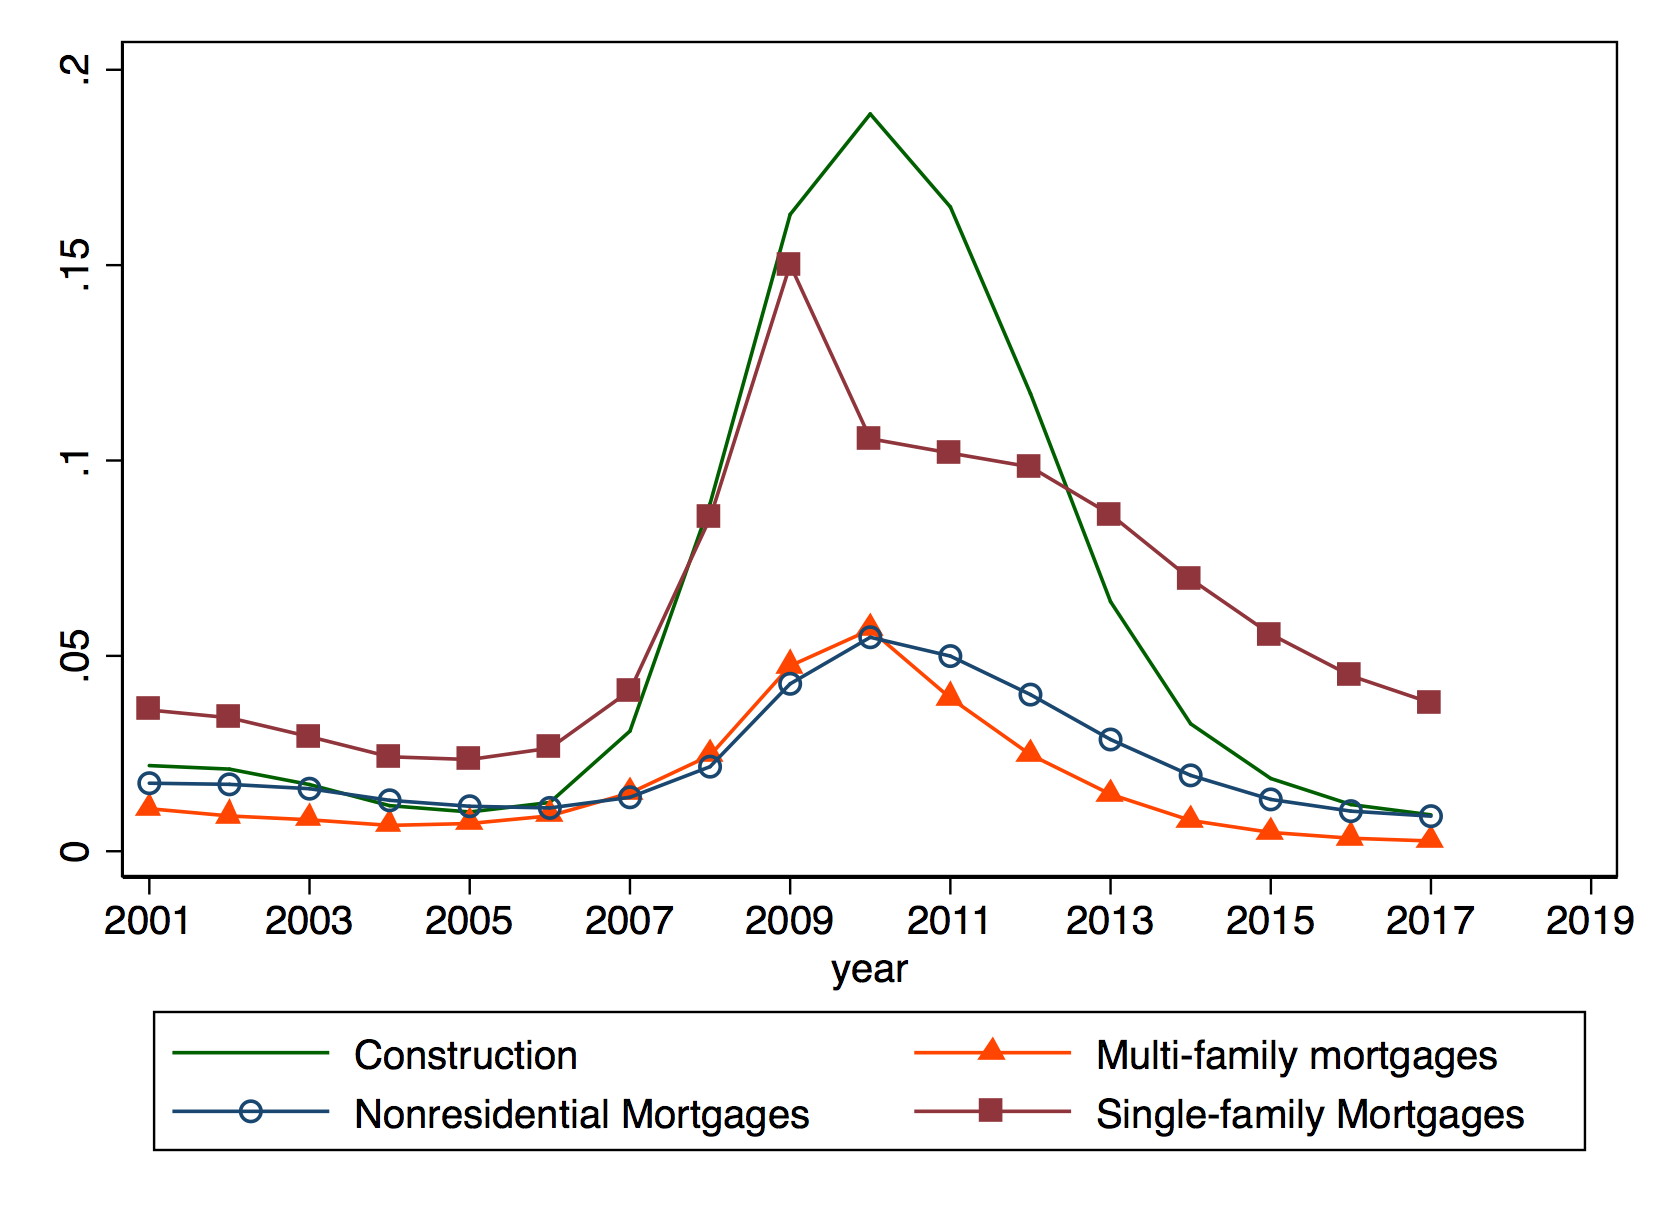
\includegraphics[width=.75\textwidth]{\dir/Delin_rates}
	\end{center}
\end{figure} 

\end{frame}


\begin{frame}{Persistent Construction}

\begin{itemize}
	\item Residential single-family construction started to fall at the beginning of 2006.\ms
	\item Commercial started to fall at the beginning of 2008. 
\end{itemize}

\begin{figure}[h!] 
	\begin{center}
		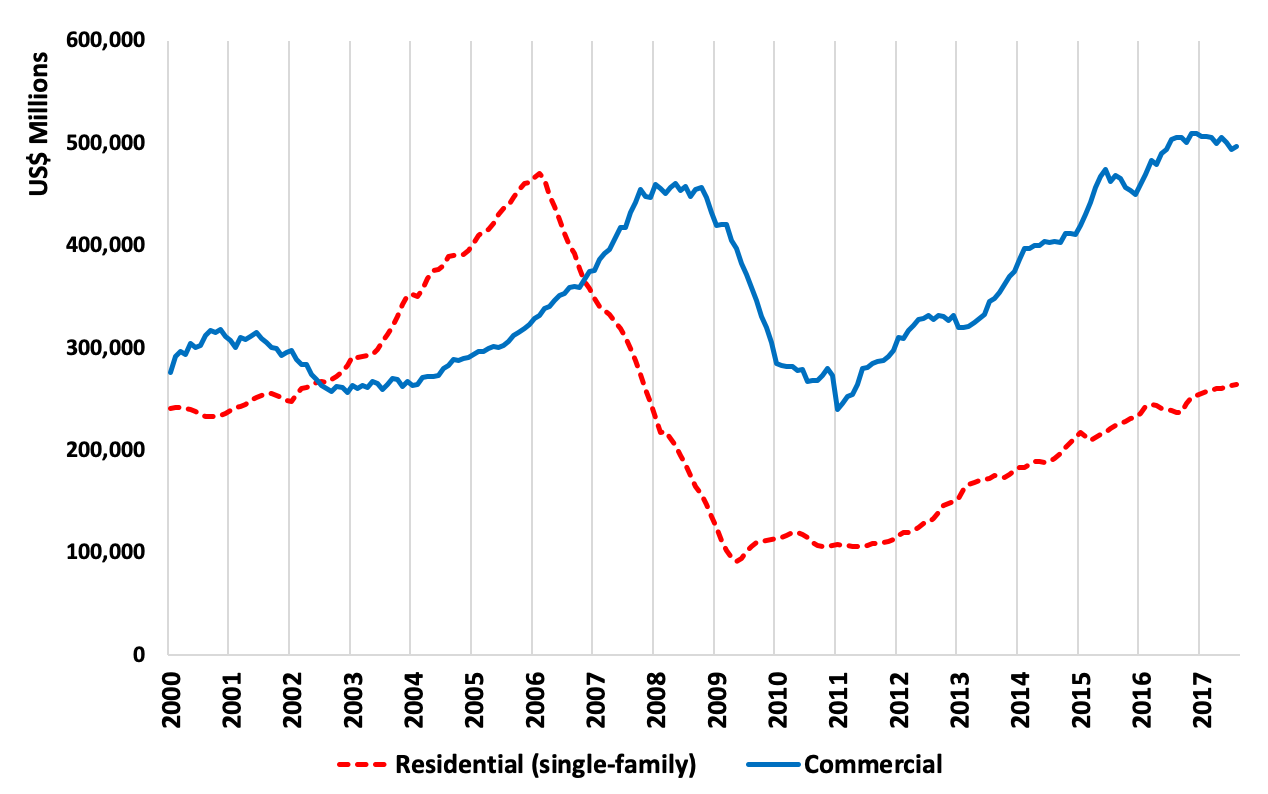
\includegraphics[scale=0.32]{\dir/Const_PiP}
	\end{center}
	\caption{Source: U.S. Census Survey of Construction}
\end{figure} 

\end{frame}

\begin{frame}
\frametitle{Relevance of the Primary Market (for Commercial)}

\begin{itemize}
	\item Share of new traded properties is around 20\% of total transactions.
	
	%	\onslide*<2>{\myitem{Important increase in transactions that occurs with the price surge.}}
	
	\item During the crisis, higher relevance of new properties sold by developers.
	
\end{itemize}

\begin{figure}[h!] 
	\begin{center}
		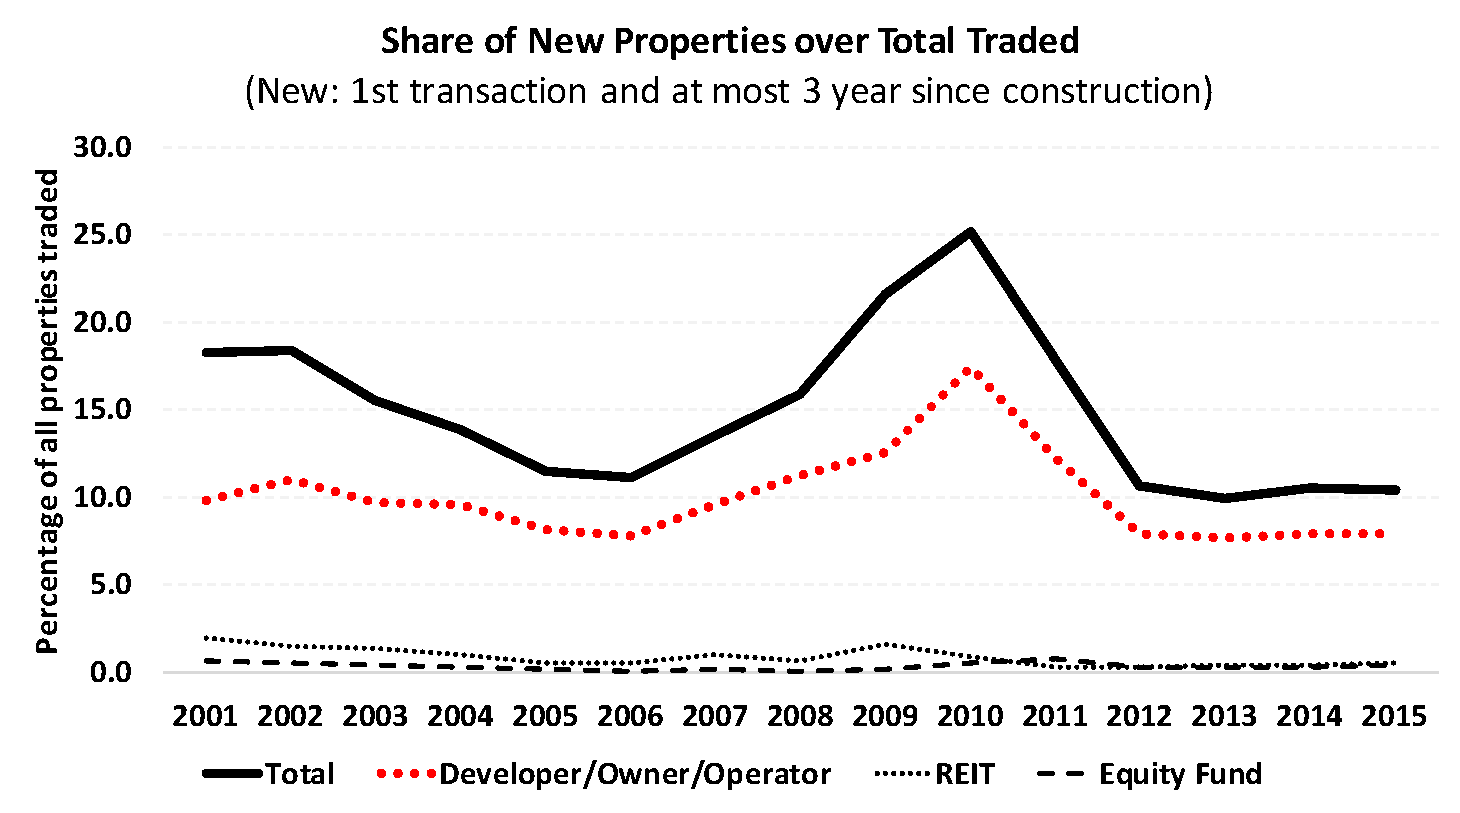
\includegraphics[width=.9\textwidth]{\dir/Shares_3y}
	\end{center}
\end{figure} 
\end{frame}

\begin{frame}{Persistent Construction: Multi-family}

\begin{itemize}
\item Residential multi-family construction started to fall in 2007.\ms

\end{itemize}

\begin{figure}[h!] 
\begin{center}
	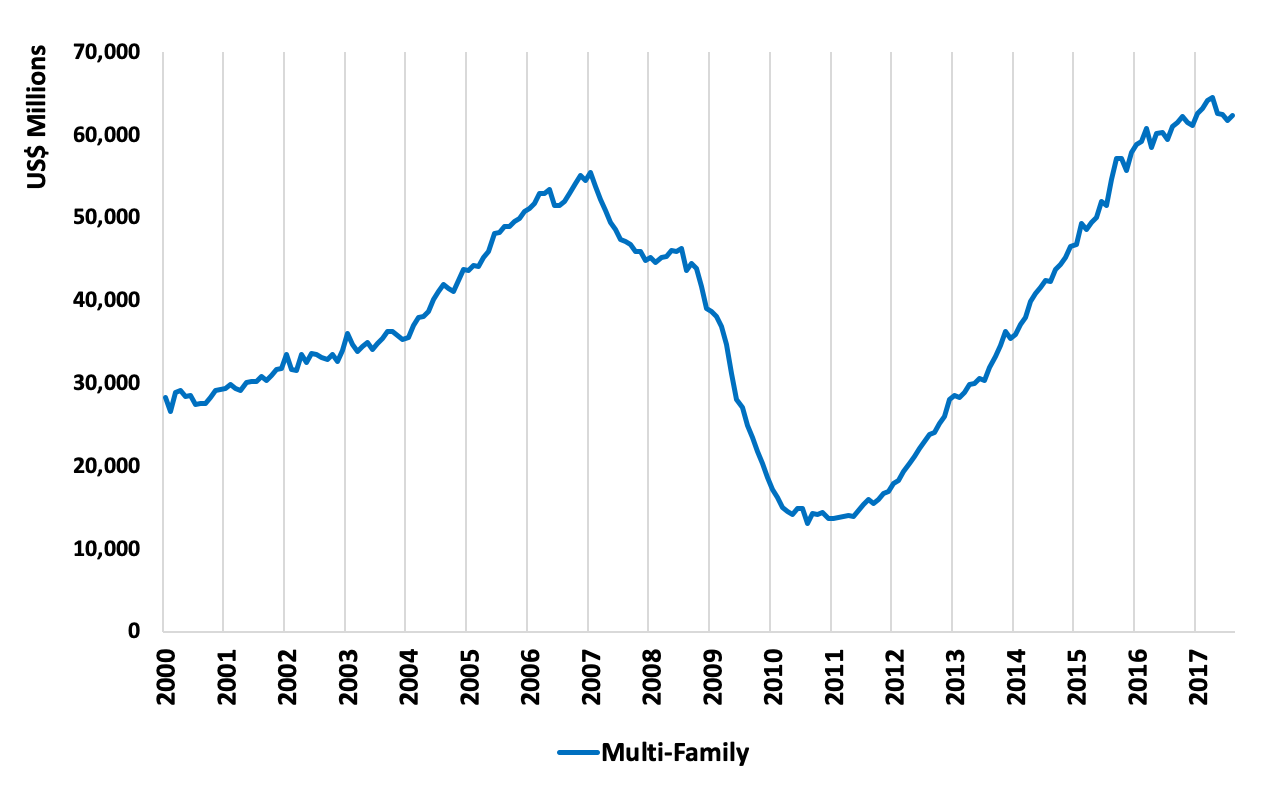
\includegraphics[scale=0.32]{\dir/Const_PiP_Multi}
\end{center}
\caption{Source: U.S. Census Survey of Construction}
\end{figure} 

\end{frame}


%---------------------------------------------------------------------- SLIDE -
\begin{frame}{TTB in the Data}{Multi-family}

\begin{itemize}
\item TTB for Building of more than 20 units went from 11 months in 2000 to 17 month in 2018.
\end{itemize}

\begin{figure}[H]
%\caption{\textbf{\small Stock Market Ratios}}
\label{Index_Construction}
\centering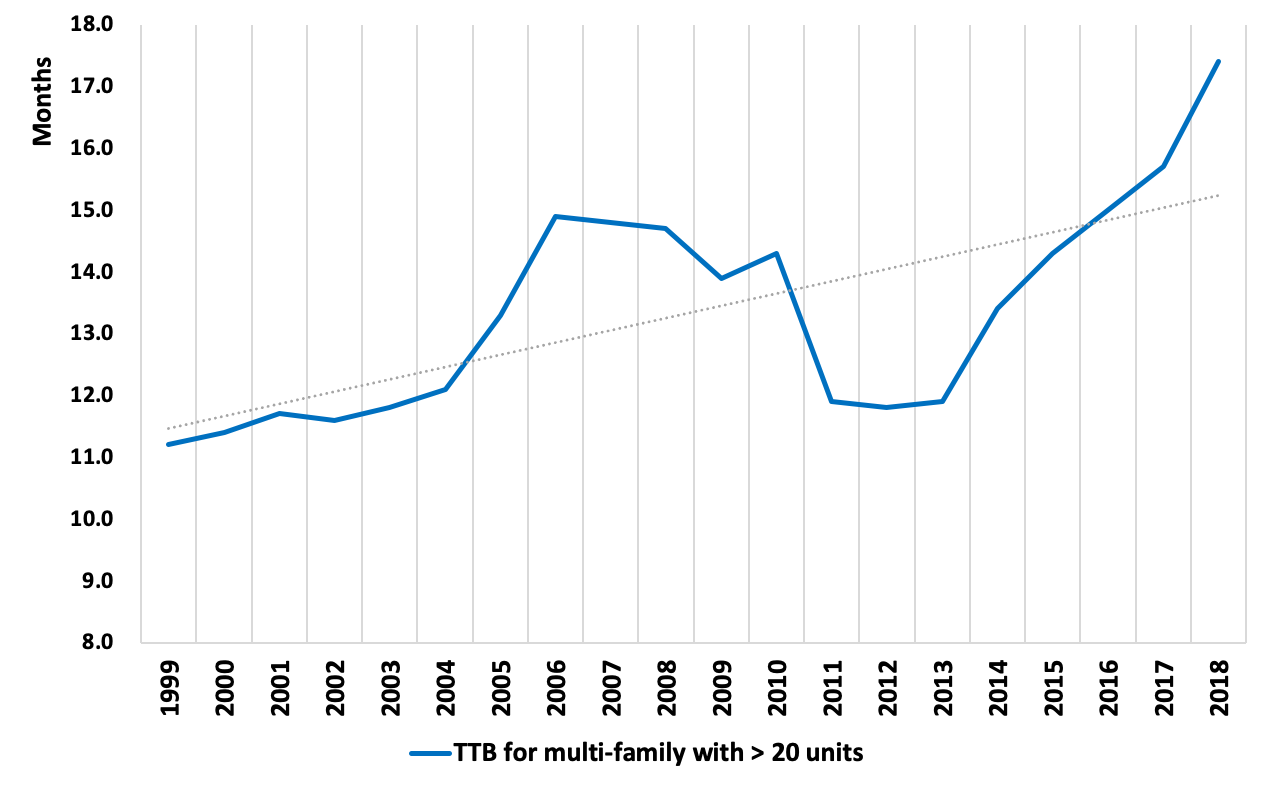
\includegraphics[scale=0.3]{\dir/TTB_residential}
\caption{Source: U.S. Census Survey of Construction.}
\end{figure}
\end{frame}


%%%%%%%%%%%%%%%%%%%%%%%%%%%%%%%%%%%%%%%%%%%%%%%%%%%%%%%%%%%%%%%
%%%%%%%%%%%%%%%%%%%%%%%%%%%%%%%%%%%%%%%%%%%%%%%%%%%%%%%%%%%%%%%
%%%%%%%%%%%%%%%%%%%%%%%%%%%%%%%%%%%%%%%%%%%%%%%%%%%%%%%%%%%%%%%
\section{Model}

%---------------------------------------------------------------------- SLIDE -
\begin{frame}
\frametitle{The Economy}

\begin{figure}[h!]
	%\caption{\textbf{\small Stock Market Ratios}}
	\label{model1}
	\centering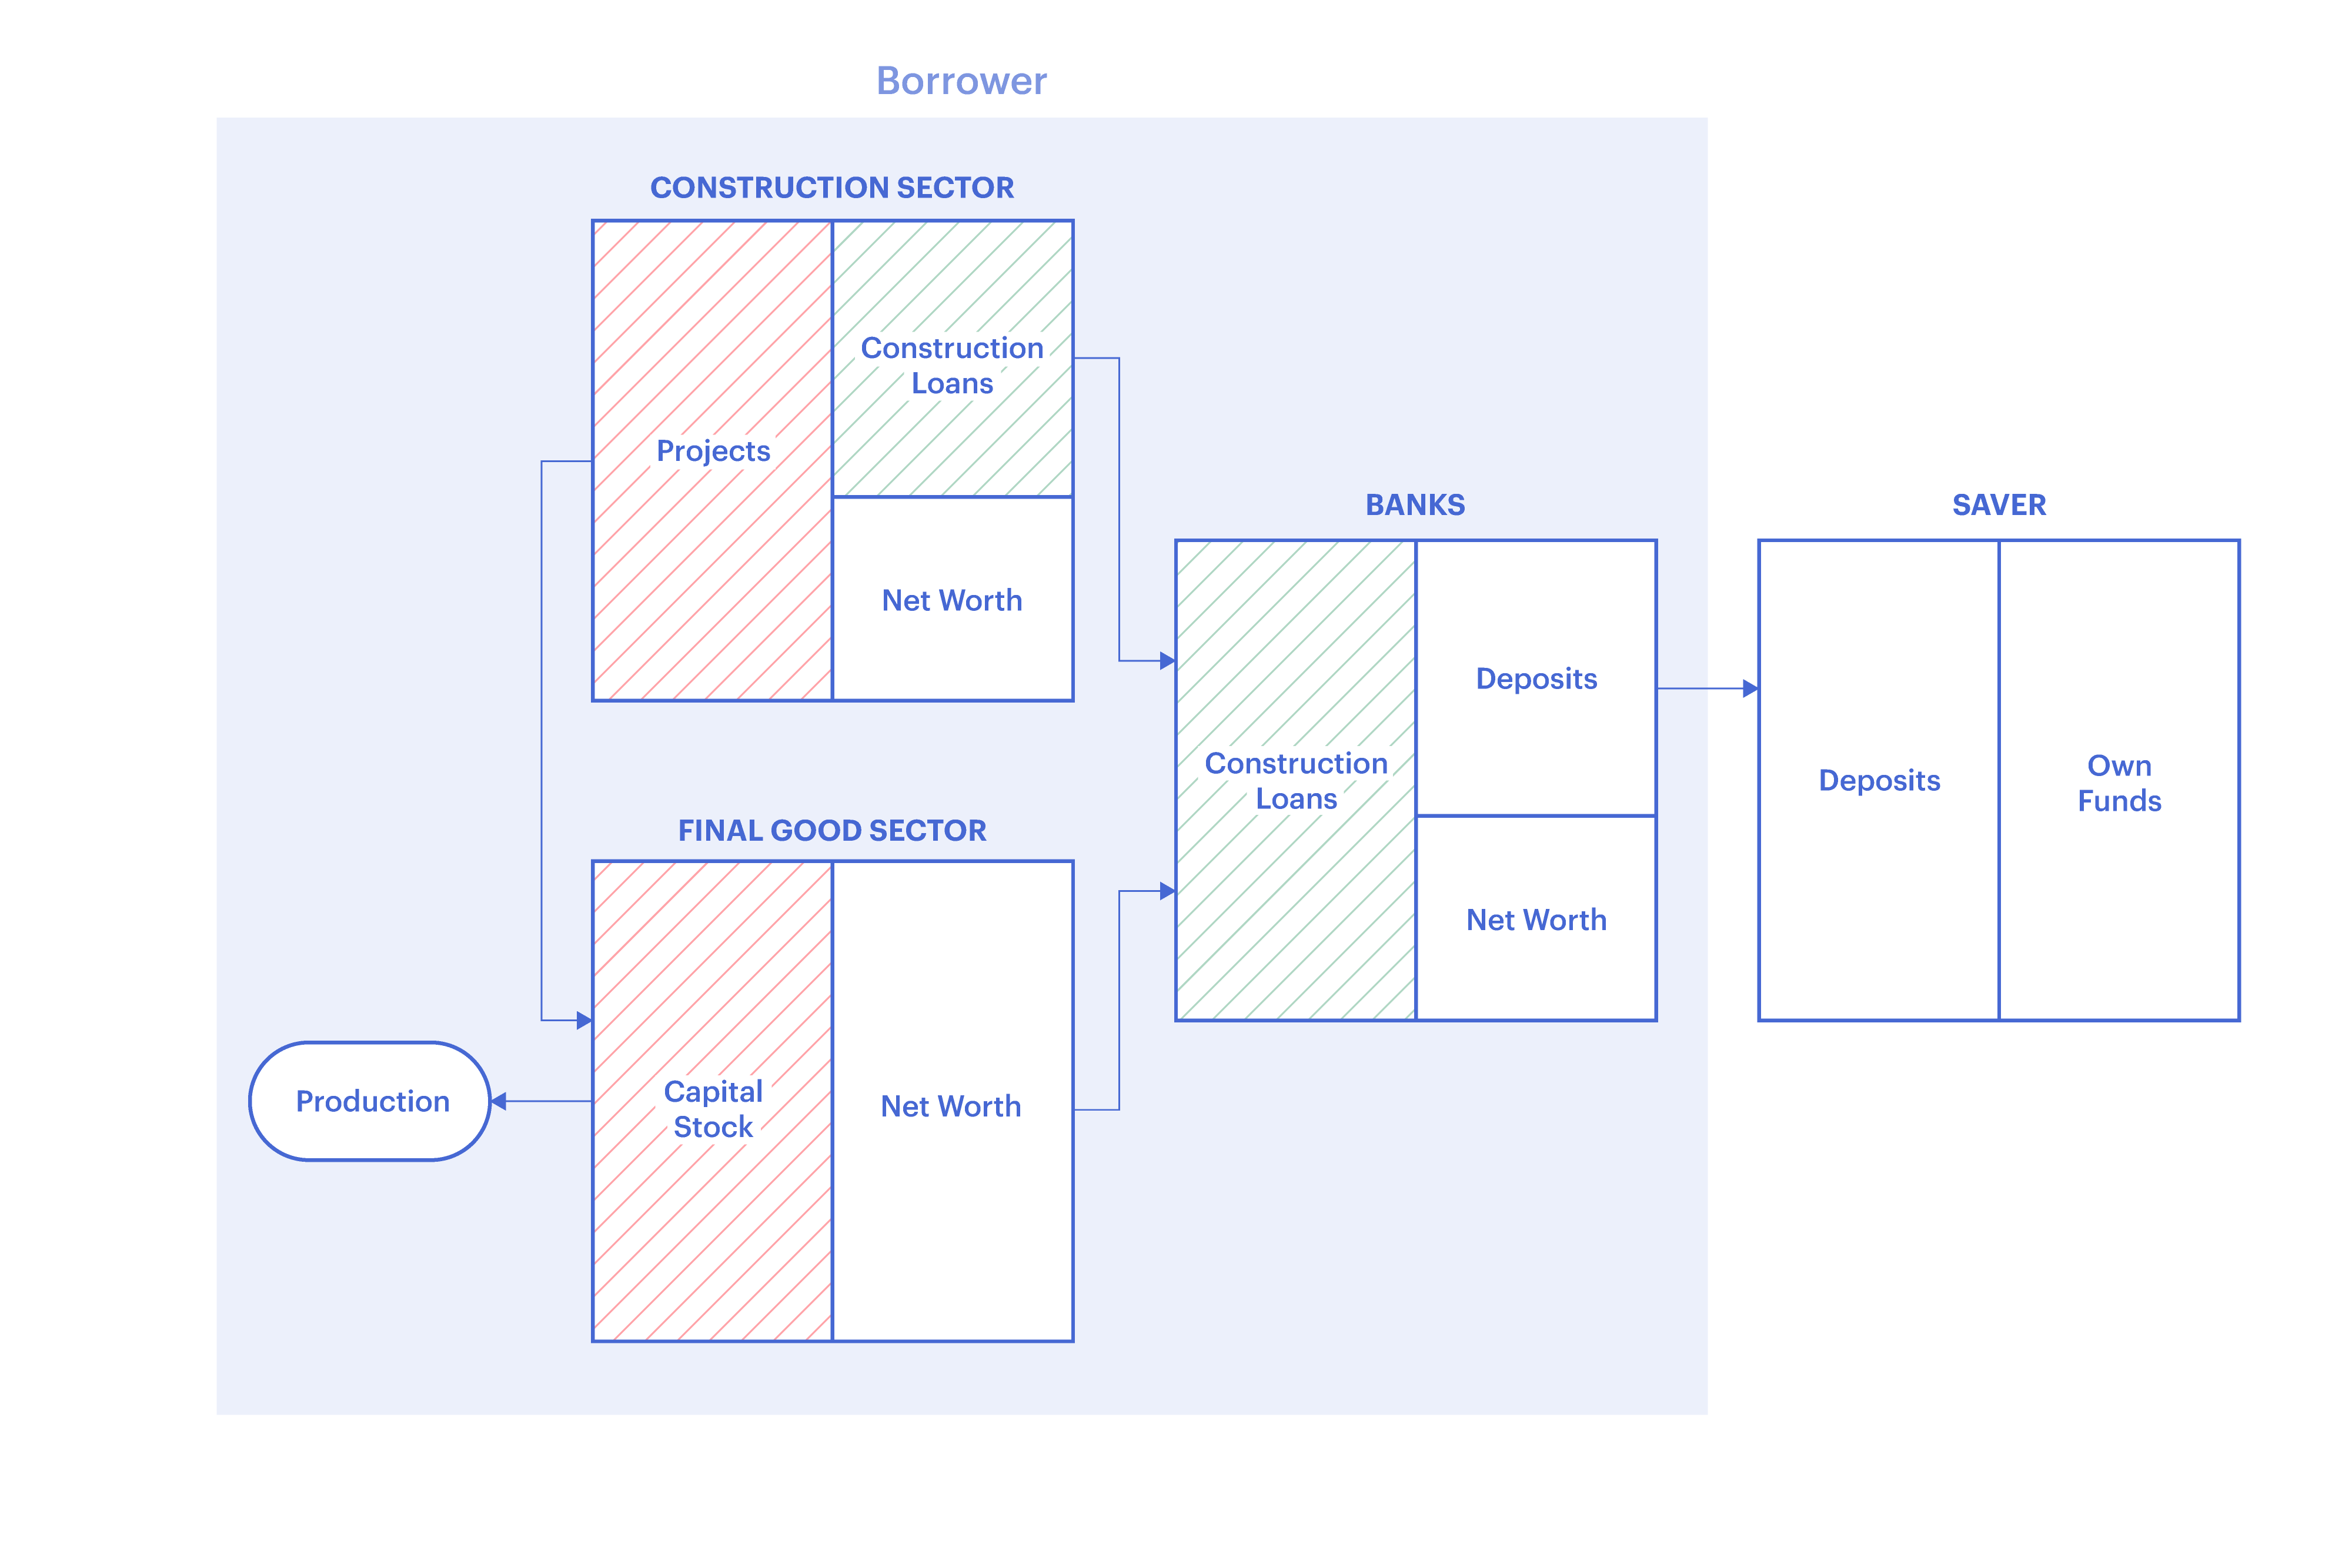
\includegraphics[scale=0.17]{\dir/model_new_partial.png}
\end{figure}

\end{frame}



%---------------------------------------------------------------------- SLIDE -
\begin{frame}
\frametitle{The Model}
\framesubtitle{Overview}

\begin{itemize}
	\item Five type of agents: two Household ($hh$), a Firm ($f$), a Bank ($b$), real estate developers ($d$) and the government ($g$).
	\ms
	\item The final good firm produces the consumption good using capital and labor. They buy capital from developers. \ms
	
	\item There are $N^d$ developers. Each developer manages $N^p$ projects.  RE developers sell real estate as capital to firm.
	\ms	
	\item To finance the creation of new capital, the developer issues \textcolor{blue}{long-term defaultable bonds}.
	\ms	
	\item Banks take deposits from the household and provide loans to the developers.
	\ms
	\item The government sell land to the developers.
\end{itemize}
\end{frame}

\begin{frame}
\frametitle{Decentralized markets}

\begin{itemize}
	\item There are 4  type of markets  markets: final good, capital goods, labor,  and  credit. \ms
	
	\item The \textbf{final good} is the nummeraire so its price is always one.  \ms
	\begin{itemize}
		\item The firm decides how much to produce and the households how much to consume. \ms
		
		\item  If demand is higher than supply, the available supply is prorated among households according ot their expressed demands. If demand is lower than supply, the good perishes and the firm only gets the demanded goods as revenue. \ms
	\end{itemize}
	
	\item In the \textbf{labor market} there are two suppliers: the saver household and the borrower household. \ms
	
		\begin{itemize}
		\item Their labor services are imperfect complements so each household chooses its wage each period. At the chosen wage, they will supply as much labor as demanded. Households get a disutility from labor. \ms
		
		\item  I will assume that real estate developers only hire labor from the saver household and the final good firm hires labor from both. \ms
	\end{itemize}
	

\end{itemize}
\end{frame}

\begin{frame}
\frametitle{Decentralized markets (continued)}

\begin{itemize}

	
	\item  In the \textbf{credit market}, the bank will provide a different long-term interest rate for each developer and a different roll-over interest rate for each project. \ms
	\begin{itemize}
		\item  Instead of directly choosing the long-term interest rate for each developer, the bank chooses the parameters of a pricing function that takes as input the developers current net worth and the average leverage of its projects. \ms
		
		\item Analogously, for the roll-over interest rate of each project the bank determines the parameters of a pricing function that takes as input the leverage of the project, the stage of the project, the net worth of the developer and the average leverage of the developers' projects. . \ms
		
		\item Also, each period the bank determines a maximum amount of loans available for new projects. \ms
	\end{itemize}

	\item In the \textbf{capital goods} market, I assume that each developer produces a different capital good, and the final good firm bundles the different capital goods.  \ms
	
	\begin{itemize}
		\item At each period, developers choose the price of their capital good and expose an inventory to the market. If the final firm demands less that the inventory, the remaining capital is depreciated and stays as inventory.
	\end{itemize}
	
	

\end{itemize}
\end{frame}


\begin{frame}
\frametitle{RE developers' problem}
\framesubtitle{Construction process}
\begin{itemize}
	
	\item There are $N^d$ developers indexed by $i$ and each manages $N^p$ projects indexed by $j$. \ms
	
	\item Each project needs to go through $N^{TTB}$ stages.  At stage 0, the developer decides whether to start a project or not. If it starts, he decides how much land $X_{ij}$, labor  $L_{ij}$, and debt $M_{ij}$ to take. \ms
	
	\item The amount of debt can only be a fraction $\lambda^d$ of the total cost of the project. 
	
	\item The scale of the project upon completion is $K^d_{ij,t} = Z^d_{ij,t} X^{\alpha^d}_{ij,t} L^{1-\alpha^d}_{ij,t}$ where  $Z^d_{ij,t}$ is a project specific quality shock. \ms

 	\item The shock follows an $AR(1)$ process. At each stage, the developer observes a realization of the shock. \ms
	
	\item At stages $1,...,N^{TTB}$, the developer decides whether to advance, stay put, or default. Hence, the stage of the project may differ from the age of the project. \ms
	
	\item Each period, developer $j$ chooses price $p^k_{j}$.
	
	
\end{itemize}

\end{frame}

\begin{frame}
\frametitle{RE developers' problem}
\framesubtitle{Debt and State Variables}
\begin{itemize}
	
	\item Debt needs to be paid at age $N^{TTB}$. If the project is not finished, the developer can roll-over the debt at the roll-over interest rate $i_{ij,t}^{RO}$.\ms
	
	\item If the developer decides to default, he has to pay a default penalty of $\phi^D$. \ms
	
	\item Upon completion or default, the developer has the option to start a new project. \ms
	
	\item \textbf{Project-level states:} For each project, the developer observes the stage $s_{ij,t}$ the age $a_{ij,t}$ of the project, the amount of debt $M_{ij,t}$ the amount of land $X_{ij,t}$, the amount of labor $L_{ij,t}$, the roll-over interest rate $i^{RO}_{ij,t}$ interest rate and the quality shock of the project $Z^d_{ij,t}$. \ms
	
	\item \textbf{Developer-level states:}  Each developer observes the long-term interest-rate $i^M_{i,t}$, the stock of capital goods $K^f_{i,t}$ owned by the final good firm and the cumulative of projects at each stage $s$ by other developers $K^s_{t}$ . \ms
\end{itemize}

\end{frame}

\begin{frame}
\frametitle{RE developers' problem}
\framesubtitle{Net worth and Objective function}
\begin{itemize}
	
	\item Each project generates a cost equal to $C_{ij,t}=\sum_{j=1}^{N^p} \left(L_{ij,t} w^S \iota(s_{ij,t})) + p^X_t X_{ij,t} \mathbb{1}_{\{s_{ij,t}=0\}}\right)$ where $\iota(s_{ij,t}))$ is the fraction of the total labor that is sued in stage $s$. \ms
	
	\item Revenue for each producer is $R_{i,t} = p^k_{i,t}   \min(K^f_{i,t} , \sum_{j=1}^{N^p} K^d_{i,j} )$. \ms
	
	\item The developer pays a dividend equal to $\text{div}^d_{i,t} = \phi n^d_{i,t}$ where $n^d_{i,t}$ is its net worth.. \ms
	
	\item The developer starts with an initial level of net worth $n^d_{i,0}$. The evolution of net worth is  
	
	\begin{align*}
	n^d_{i,t+1}=n^d_{j,t}+R_{i,t}-\sum_{j=1}^{N^p} C_{ij,t} - \text{div}^d_{i,t} 
	\end{align*}
	
	\item The developer maximizes the discount sum of expected dividend payments. 
	
	\item {\color{red} to do: treatment of risk and taxable profits.}
\end{itemize}

\end{frame}

%---------------------------------------------------------------------- SLIDE -
\begin{frame}
\frametitle{The Firm (f)}
\begin{itemize}

	\item The firm produce the final good using a Cobb-Douglas technology:
	\begin{align*}
	Y_t = Z^f_t\left(K^f_t \right)^{\alpha^f} \left(L^f_t\right)^{1-\alpha^f}
	\end{align*}
	
	where $Z^f_t$ follows a two state markov process with transition probability $\mathcal{P}$, $K^f_t$ is a bundle of capital goods and $L^F$ is labor. \ms 
	
	\item 	The aggregate TFP shock translate into \textcolor{red}{demand shocks} to RE developers. \ms
	
	\item Capital goods are bundled as $K^f_t = \sum_{i=1}^{N^d}K^{\gamma}_{j,t}$. The two types of labor are bundles as $L^f_t = {L^S}^{\gamma^s}_t  {L^B}^{\gamma^b}_t$
	
	\item The firm observes $p^k_{j,t}$ fixed by each developer $j$ and chooses $I^f_{j,t}$. The evolution is:  \ms
	\begin{align*}
	K_{j,t+1}^f = I_{j,t}^f + \p{1-\delta}K_{j,t}^f \qquad \text{for} \qquad j\in [1,...,N^d]
	\end{align*}
	
\end{itemize}

\end{frame}


%---------------------------------------------------------------------- SLIDE -
\begin{frame}[label=F]
\frametitle{The Firm}
\begin{itemize}
	
	\item Accounting  profits for tax purposes are:	 \ms
	\begin{align*}
	\Pi^{F,\tau}_t = Y^{hh}_t-w^S_t L^S_t-w^B_t L^B_t-\sum_{j=1}^{N^d} \left( \delta_j p^k_{j,t} K^f_{j,t}-bp_{j,t}^k I_{j,t}^f \right)
	\end{align*}	
	where $b$ is the fraction of new real estate that qualifies as \textit{bonus depreciation}. \ms
	
	\item Economic profits are: 
	
	\begin{align*}
	\pi_{t}&= Y_t - w_t L^F_t -\sum_{j=1}^{N^d} p^k_{j,t} I_{j,t}^f -  \tau^\pi\Pi^{F,\tau}_t 
	\end{align*}	
	
		\item The firm pays a dividend equal to $\text{div}^f_t = \phi n^f_{t}$ where $n^f_{t}$ is the net worth of the firm. The initial level of net worth  is $n^d_{i,0}$. The evolution of net worth is  
	
	\begin{align*}
	n^d_{i,t+1}=n^d_{j,t}+\pi_t- \text{div}^f_{t} 
	\end{align*}
	\item  The firm  maximizes the discount sum of expected dividend payments. 
	\ms
	
\end{itemize}


\end{frame}

\begin{frame}[label=B]
\frametitle{The Bank}
\begin{itemize}
	
	\item The bank enters a period with an amount of deposits $B_t$ and amount of loans it has provided $M_t$. \ms
	
	\item  Also, he holds an inventory of land $X^b_t$ and an inventory of capital goods $\{K^b_{i}\}_i$ that he has received from defaulted projects and has been unable to sell. \ms
	
	\item Each period, the bank chooses: \ms
	
	\begin{itemize}
	 \item The interest rates on deposits $i^B_t$ and the parameters for functions $i^M_t()$ and  $i^{RO}_t ()$.
	 
	 \item The maximum amount of new lending $\hat{M}^{\max}_t$.
	\end{itemize}

	\item When a project $j$ defaults: \ms
	
	\begin{itemize}
		\item If the project was not finished, he received a fraction $1-\xi$ of the land: $(1-\xi) X_j$. $\xi$ represents the deadweight loss of the process. \ms
		
		\item If the project was finished, he receives a fraction of the capital good: $(1-\xi) K_{i,t}$.
\end{itemize}
	
	
\end{itemize}
\end{frame}

\begin{frame}[label=B]
\frametitle{The Bank (continued)}
\begin{itemize}
	
	\item The bank has a regulatory constraint on the stock of loans it holds:
	
	$$M_t \leq \lambda (B_t+n^b_t)$$
	
	where $n^b_t$ is the net worth of the bank.
	
	\item Let $M^d$ be the total amount of payments received from developers. The evolution of net worth is:
	
	\begin{align*}
	n^b_{i,t+1}=n^b_{j,t}+B_{t+1}+M^d_t -(1+i^B_t )B_t - \hat{M}_t - \text{div}^f_{t} 
	\end{align*}
	
	
	\item {\color{red} to do: include proceedings from foreclosures and taxes, define risk preferences}.
	
\end{itemize}
\end{frame}

%---------------------------------------------------------------------- SLIDE -
\begin{frame}
\frametitle{The Household, the Government and shocks}
\begin{itemize}
	
	\item The saver household consumes the final good, supply labor to the final good and RE sector, and deposits its saving in the banks.  \ms
	
	\item The borrower consumes the final good, supply labor to the final good and receives dividends from the the developers, the firms and the banks. \ms
	
	\item Both households have GHH preferences over consumption and labor. They pay labor taxes and receive government transfers. \ms
	
	\item The government supply one unit of land each period and fixes a price $p^x_t$. In the case that not all the supply is sold, it holds an inventory. In addition, it collect taxes and provides transfers to the households according to their population shares. \ms

\end{itemize}

\end{frame}

%---------------------------------------------------------------------- SLIDE -

%---------------------------------------------------------------------- SLIDE -
\begin{frame}
\frametitle{Shocks}
\begin{itemize}
	
\item There are three aggregate shocks that follow two state markov processes: \ms

\begin{itemize}
	\item TFP shock in the final good sector $Z^f_t$ \ms
	
	\item Volatility shock to the idiosyncratic quality shock of the developers $\sigma_{Z^d}$.\ms
	
	\item Shock to financial conditions $\{\lambda^b, \lambda^d\}$.
\end{itemize}
\end{itemize}

\end{frame}

%---------------------------------------------------------------------- SLIDE -
\begin{frame}[noframenumbering]
\frametitle{Final Goal}

\begin{figure}[h!]
	%\caption{\textbf{\small Stock Market Ratios}}
	\label{model2}
	\centering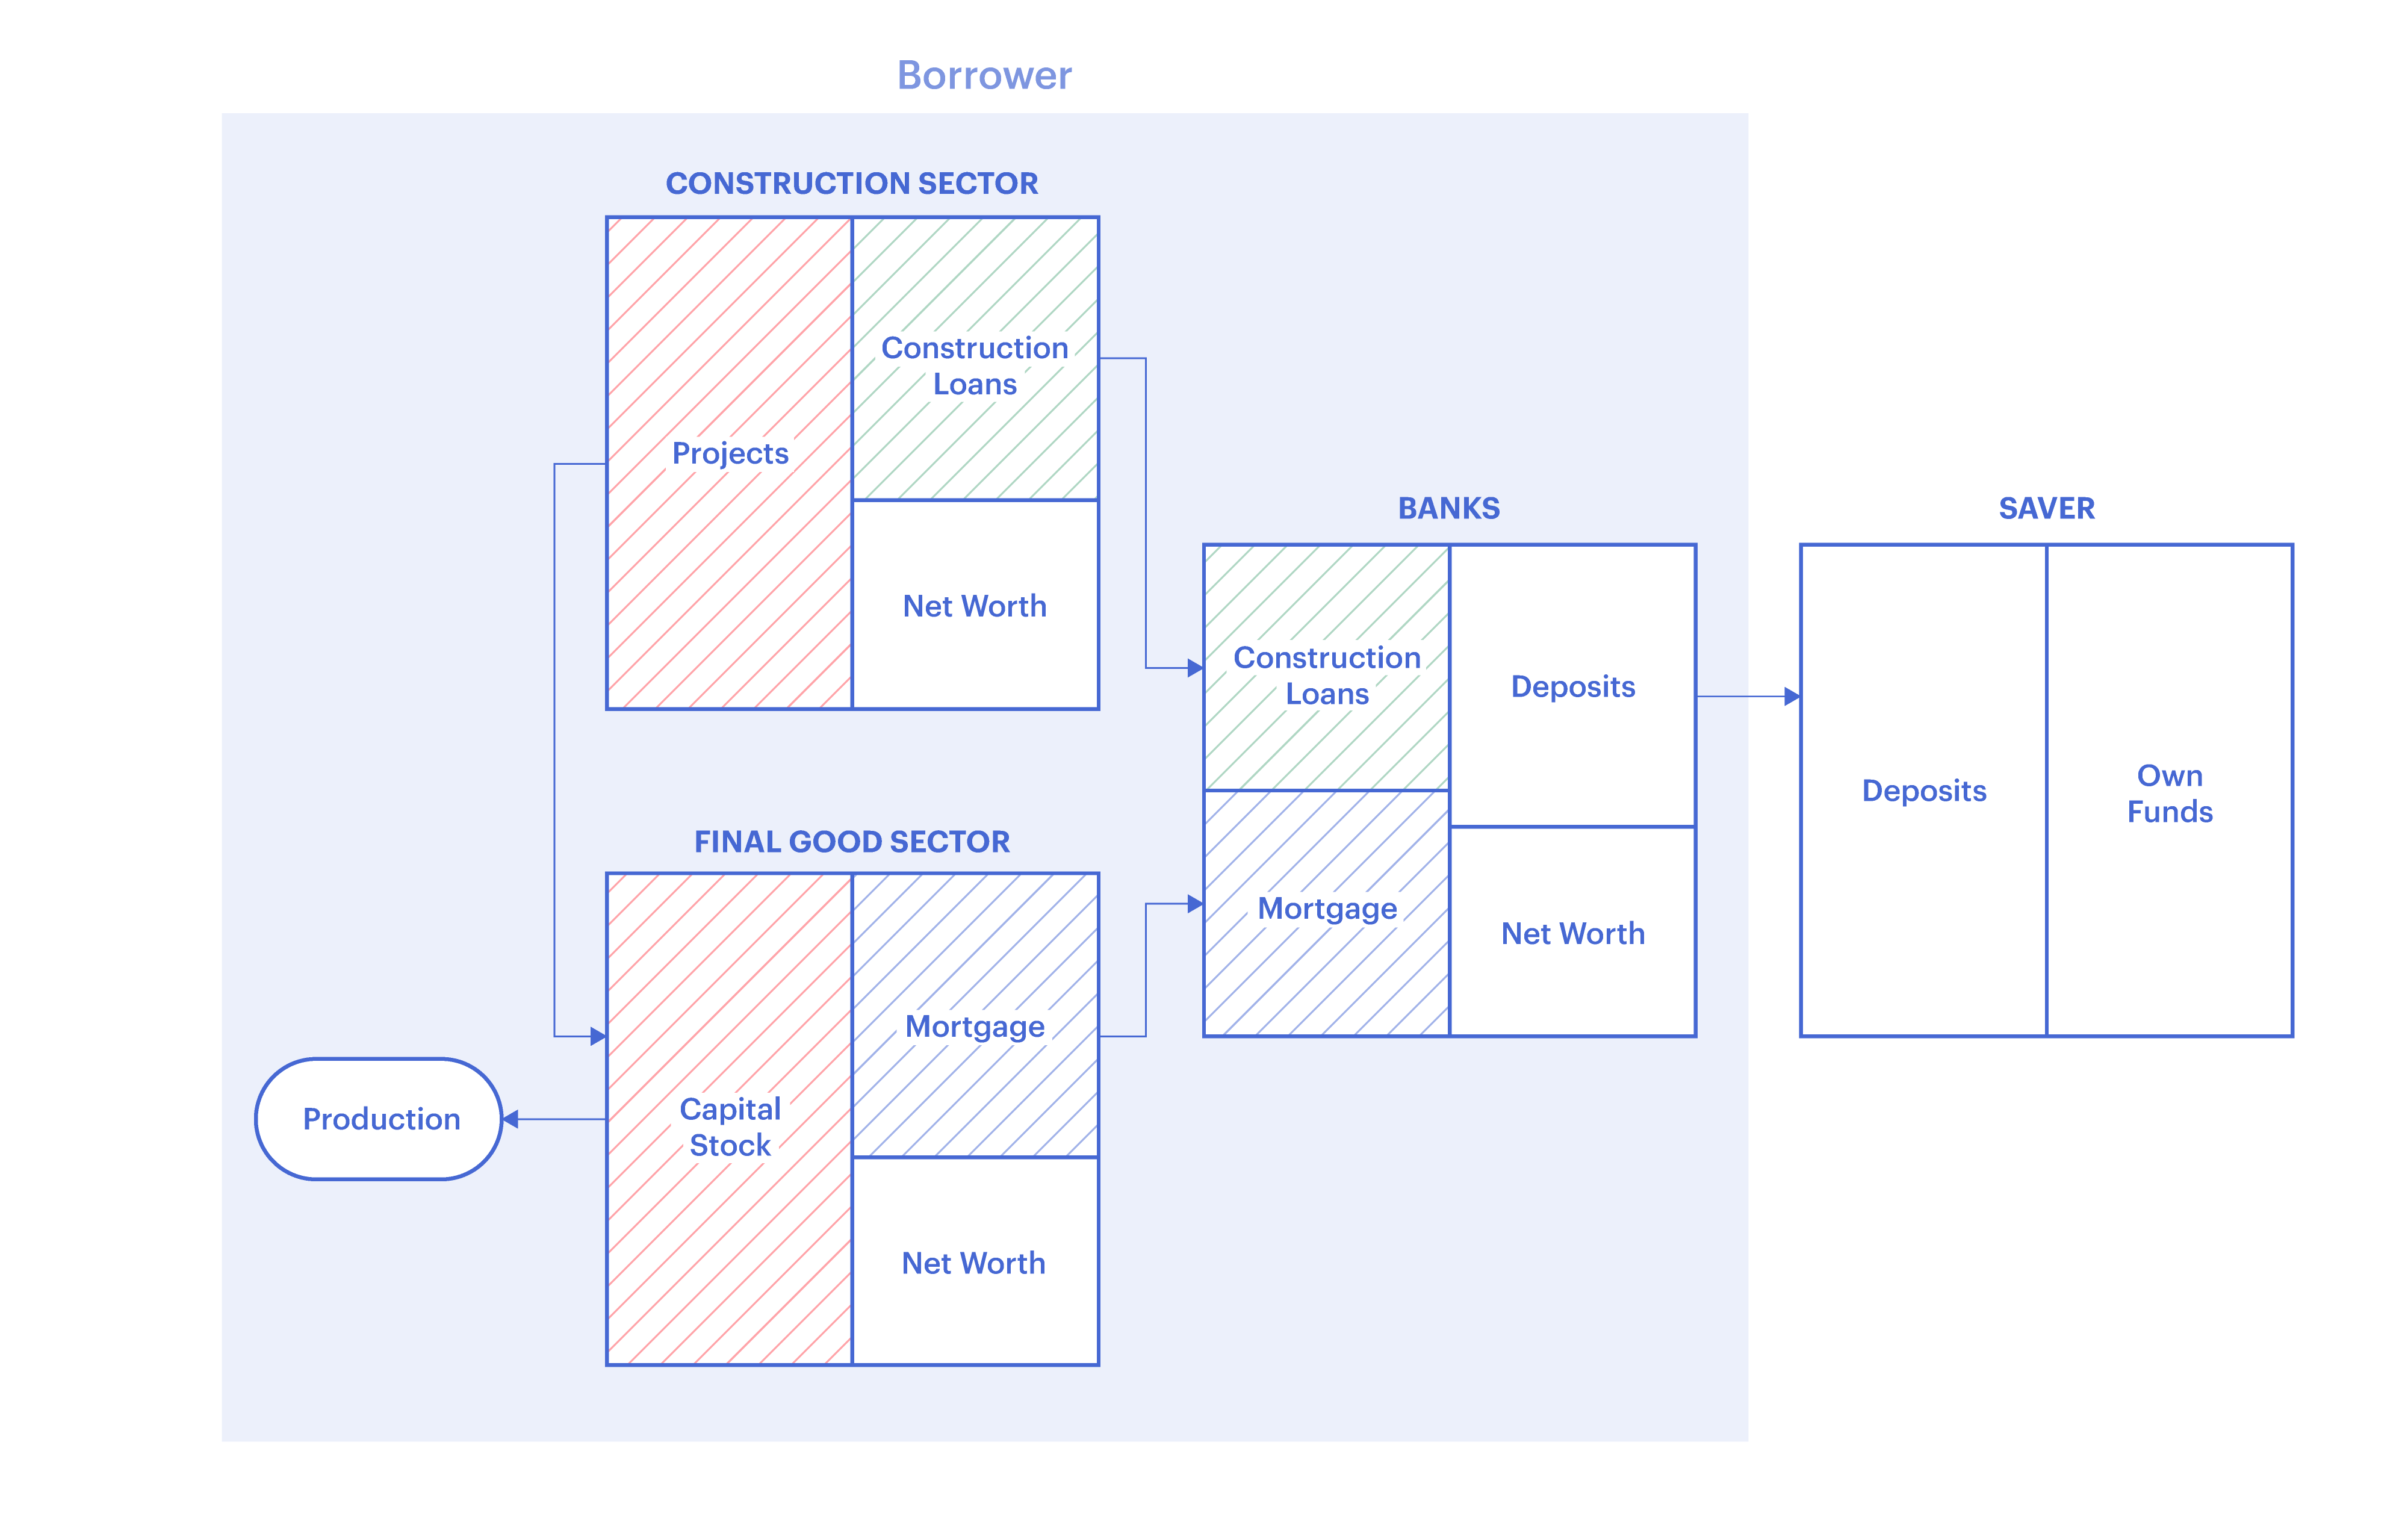
\includegraphics[scale=0.17]{\dir/model_new_full.png}
\end{figure}

\end{frame}


\end{document} 